\section*{Introduction}

Learning continuous, smooth, functions is a key problem in machine learning, as many problems
are framed as finding good interpolations between a few data points, where we define continuity as $\lim\limits_{x\to c}f(x) = f(c)$.
The continuity of a learned model is not guaranteed, and is enforced through regularization of the output, either by having enough training samples in a short time, or
using regularization such as total variation across time. Since consistency is dependent on data and regularization and cannot be guaranteed, it is empirically demonstrated. This leads to difficulties in interpolating between sparse training data, and the possibility for sudden changes in output between training points, such as suddenly jumping from one frame to the next in a learned video.
To enforce continuity, we are interested in recovering functions which guarantee $C^0$ continuity. $C^0$ continuity is a useful property for many tasks, such as in reconstructing movement to ensure that an object cannot warp between two points instantaneously. We are also interested in $C^1$ continuity, or that the derivative of a function is continuous on some domain. This is because it is not physically possible for an object to instantly change its velocity, therefore reconstructions must have $C^1$ continuity for plausible movement.

To demonstrate how to construct functions with these properties, we tackle the problem of dynamic scene reconstruction using NeRF~\cite{mildenhall2020nerf}, which is a recent method for reconstructing scenes. Following previous work, we define a static scene, which is referred to as the canonical scene, and a model which can produce deformations to the canonical scene. Our approach is a small modification to prior work: to represent the canonical scene, we use a NeRF~\cite{mildenhall2020nerf}, and the deformation model used to model movement is our proposed learned approach. The use of deformation networks has been shown to be effective at reconstructing synthetic scenes with movement as in D-NeRF~\cite{pumarola2020dnerf} and real scenes in NR(non-rigid)-NeRF~\cite{tretschk2021nonrigid}. These works show convincing
reconstructions of moving scenes, allowing for novel view synthesis from video. These methods do not have an analytic form, relying purely on learned components, but we would like to be able to analyze and modify the movement. For example, an application may want to cluster movement, or change directions, but prior work does not immediately provide a method for doing so. In contrast, classical animation tools are designed to allow for control of movement, but their use has not been explored in prior work.

To this end, we look to existing tools in animation for creating realistic movement while allowing a high-degree of control for artists and animators. For example, there are tools such as keyframing and splines, which allow animators to construct movement with a small set of tunable knobs. Despite few degrees of freedom, these tools allow artists and animators to breathe life into animation with a high degree of control. In addition, mathematical constructs such as splines have also been thoroughly studied to understand their behaviour and how they can be manipulated, and thus are readily modifiable in post-processing.

Thus, we use the animation techniques of Bezier splines as a method to enforce continuous interpolation in Dynamic NeRF, finding that we are able to get comparable performance without additional cost in memory, and the desired properties of $C^0, C^1$ continuity.
In summary, our contributions are as follows:

\begin{enumerate}
    \item A general architecture for $C^0, C^1$ continuity over a continuous domain.
    \item An application of this architecture, building on NR-NeRF to enforce continuity of movement with an analytic form with negligible computational cost, while performing on par with the original.
\end{enumerate}

\begin{figure}
    \vspace{-6mm}
    \centering
    \begin{minipage}[c]{0.5\textwidth}
    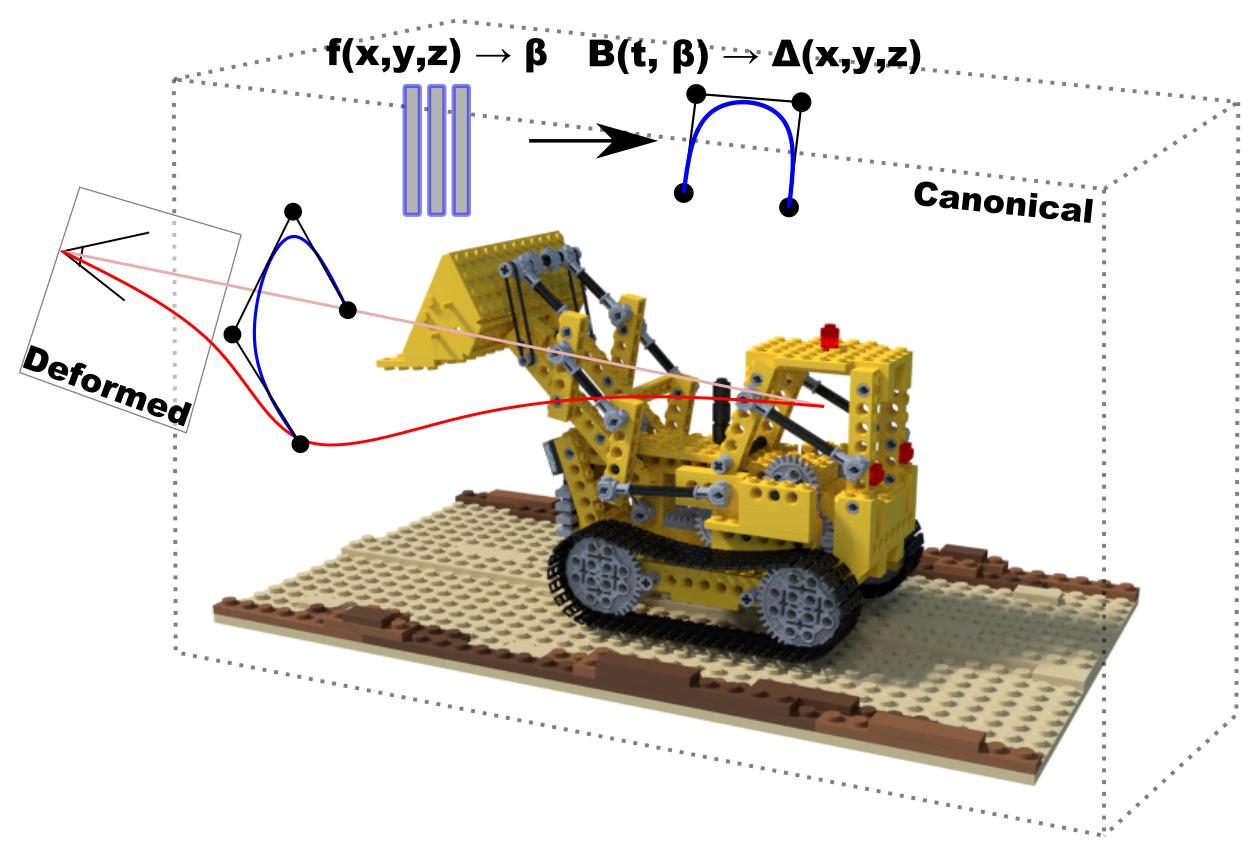
\includegraphics[width=\textwidth]{spline_nerf_diagram.png}
    \end{minipage}
    \begin{minipage}[c]{0.45\textwidth}
    \caption{
        \label{fig:arch_diagram}
        \textbf{Spline-based Dynamic NeRF}. Instead of using an MLP to directly predict ray-bending, $x' = \Delta(\text{MLP}(x, t)) + x$,  at a given time, we predict a set of Bezier spline control points. Then, we use the Bezier spline defined by these points to interpolate position based on time: \newline $x' = \Delta(B(\beta,t)) + x$, where $B$ is a Bezier spline parametrized by $\beta = \text{MLP(x)}$.
    }
    \end{minipage}
    \vspace{-10mm}
\end{figure}
